\interfootnotelinepenalty=10000
Using the LOFAR software installation described in \cite{mechev17}, we processed a typical LOFAR SKSP observation\footnote{LOFAR Observation ID L658492, co-ordinates [17h42m21.785, +037d41m46.805] observed by the LOFAR High Band Array for 8 hours between 2018-06-20 and 2018-06-21.}, while changing the averaging rate  in time and frequency. Changing these averaging parameters will change the final data size (with the data sizes studied shown in Table \ref{table:averaging}). We test the processing time for different averaging parameters by running 15 runs per parameter step. 

The data used by the LOFAR surveys is archived at a time resolution of 1 second intervals and frequency resolution of 16 channels per subband (equivalent to 12kHz channel width). While some of the processing steps such as flagging of Radio Frequency Interference and removal of bright off-axis sources produce better results when performed on the high-resolution data, later steps can be performed on averaged data with little impact on the final product quality. To speed up processing, the raw data is averaged in time and frequency, decreasing the input data size to later tasks. The main aims of the LoTSS survey can be accomplished if the final data products from the \texttt{prefactor} pipeline are averaged to a time resolution of 8 seconds per sample and frequency of 2 channels per subband. These averaging parameters correspond to a reduction in data size by a factor of 64. Nevertheless, other science cases require less averaging of the data. Our aim is to understand how the processing of this larger data will scale. To measure the scalability of processing, we measure the performance of the \texttt{prefactor} pipeline for data sizes between the raw data of 64GB/subband and the averaged data of 1GB/subband. The tested data sizes and parameters are shown in table \ref{table:averaging}, and discussed in Section \ref{sec:ch6_results_size}.

We performed the scalability tests on a dedicated node of the SURFsara \texttt{GINA} cluster, f18-01. The node is a typical hardware node used by our production LoTSS processing, however it is dedicated for the tests in order to ensure there is no contamination by other software. The node is described in Section \ref{sec:ch6_hardware}. 
     
%There are two sources of latency that need to be studied for a true end-to-end model of LOFAR processing. The first is the performance of the LOFAR software on the Dutch grid for a wide range of processing parameters. The second is the overhead, such as job queuing and data movement. Both of these effects depend on similar parameters such as data size and number of CPUs used. 
%We will examine these effects in our study of the LOFAR processing performance by studying the performance at different parameter steps. While some parts of the processing software may change, the infrastructure parts of our performance model can be used independently of the the processing software and can even be applied to other scientific projects running on the \texttt{GINA} cluster. 

We processed the sample data set with the LOFAR \texttt{prefactor} pipeline. The \texttt{prefactor} version used was the same as we use for the LOFAR SKSP broadband surveys \citep{prefactor_LOTSS_DR1}. This software consists of several steps executed in sequence, shown graphically in Figure \ref{fig:ch6_prefactor_steps}. The important \texttt{prefactor} steps are as follows. The {\fontfamily{qcr}\selectfont predict\_ateam} and {\fontfamily{qcr}\selectfont ateamcliptar} steps predict the contamination by bright off-axis sources and remove these effects respectively. The {\fontfamily{qcr}\selectfont dpppconcat} step is responsible for concatenating 10 Subbands into a single file which is in turn calibrated. The step {\fontfamily{qcr}\selectfont gsmcal\_solve} is responsible for calibration of the data against a model of the radio sky. The solutions produced by {\fontfamily{qcr}\selectfont gsmcal\_solve} are used by {\fontfamily{qcr}\selectfont gsmcal\_apply} and applied to the scientific observation.

\begin{figure}
    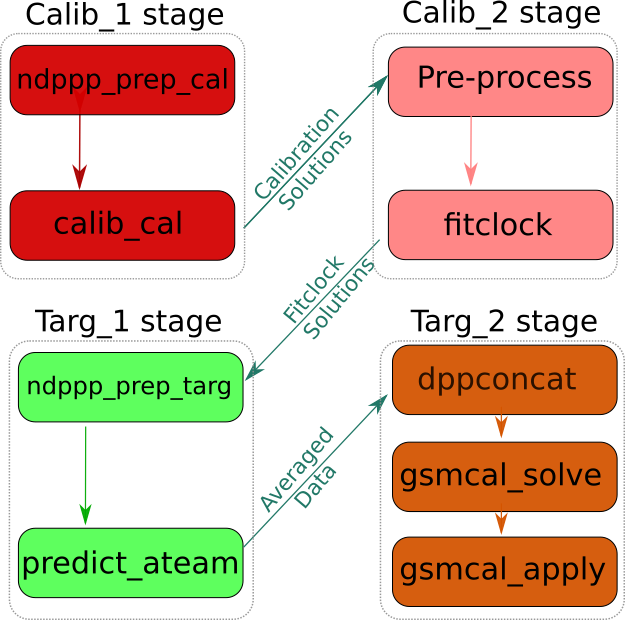
\includegraphics[width=0.8\linewidth]{ch6/figures/4_stages_steps1.png}
      \caption{The major steps of the \texttt{prefactor} DI pipeline. }
	\label{fig:ch6_prefactor_steps}
\end{figure}

\subsection{Processing Metrics}
The goal for our scalability model is to understand the effect of several parameters on the job completion time of LOFAR software. We do this by testing the processing time for various values of data size, number of CPUs used and sky model size. 
 

\begin{table}[!ht]
\centering
\begin{tabular}{||c| c | c | c||} 
 \hline
\multicolumn{1}{|p{1.7cm}|}{\centering Averaging \\ ratio} & \multicolumn{1}{|p{1.8cm}|}{\centering Time averaging \\ parameter (sec)} &  \multicolumn{1}{|p{1.7cm}|}{\centering Channels per Subband} & \multicolumn{1}{|p{1.8cm}|}{\centering Averaged \\ Size (Gb) }\\ [0.5ex]
 \hline
 \rowcolor{Gray}
  \hline
 64x & 8   & 2   &  1.235   \\ 
  \hline
 32x & 4   & 2   &  2.459   \\ 
 16x & 2   & 2   &  4.906   \\ 
 8x & 1   & 2   &  9.802   \\ 
 4x & 1   & 4   &  18.00  \\ 
 2x & 1   & 8   &  36.72  \\ 
 1x & 1   & 16   &  66.88  \\[1ex] 
 \hline
\end{tabular}
    \caption[Averaging parameters and final data sizes for a sample LOFAR Observation]{Averaging parameters and final data sizes tested for the sample LOFAR SKSP observation. The raw data is 64 GB per subband. The LOFAR SKSP data processing uses averaging parameters of 8 seconds and 2 channels per subband. This reduces the raw data by a factor of 64. We highlight the data size used in the LOFAR SKSP survey.   }
\label{table:averaging}
\end{table}

The slowest step of the \texttt{prefactor} pipeline is the {\fontfamily{qcr}\selectfont gsmcal\_solve} step, which performs the gain calibration against a model of the radio sky. This step operates on a concatenated data set that consists of 10 Subbands. We obtain the calibration model through the TGSS sky model creator\footnote{Accessible at \href{http://tgssadr.strw.leidenuniv.nl/doku.php}{the TGSS ADR portal}.}. By default this service creates a text file describing the sky-model from the TGSS survey \citep{tgssadr} as a combination of gaussians and point sources. By default, it sets a threshold of sources brighter than 0.3 Jy. 
Lowering this threshold creates longer sky-model files with more faint sources, while increasing it will return only the few brightest sources. Since sky model calibration requires converting the sky-model into modelled \gls{visibilities}\citep[e.g.][]{dppp, radio_visibility_sage,app_synth}, a longer sky model will increase the time taken to gain calibrate a data set. We created 7 sky models with a flux cutoff ranging between 0.05 Jy and 1.5 Jy. The number of sources in the resulting models are listed in Table \ref{table:skymodels}. 
For production\footnote{The query used to obtain model 3 is at the following link \url{http://bit.ly/tgss_model}}, we used the minimum sensitivity parameters for model 3.
%%%%%Each line of these model files corresponds to one source, modelled either as a point or an ellipse), hence the second column also lists the number of sources per sky model file. %Suggested remove by Huub

It is important to note that the complexity and accuracy of the sky model depend on the direction of observation and the ionospheric conditions in which the observation was performed. As such, our test is only a heuristic for predicting the run-time based on the calibration model length. Additionally, it is notable that the number of sources is exponentially dependent on the minimum sky model sensitivity (seen in Figure \ref{fig:ch6_skymodel_size}, more in \citealt{tgssadr,Wendy_bootes}). According to this relationship, even a modest decrease in sensitivity cutoff can significantly decrease the size of the model.

\begin{table}[!ht]
\centering
\begin{tabular}{||c| c | c||} 
 \hline
 Sky model \# & min sensitivity & \# sources  \\ [0.5ex] 
 \hline
 model 1 & 0.05 Jy & 809    \\ 
 model 2 & 0.1 Jy & 503   \\
 \rowcolor{Gray}
  \hline
 model 3 & 0.3 Jy & 180   \\
  \hline
 model 4 & 0.5 Jy & 96  \\
 model 5 & 0.8 Jy & 49   \\ 
 model 6 & 1.0 Jy & 34   \\
 model 7 & 1.5 Jy & 16   \\[1ex] 
 \hline
\end{tabular}
    \caption[List of test sky models]{List of test sky models. Model 3 is created with the parameters used in our production processing of LOFAR data. All models include objects within 5 degrees from the centre of the pointing.  }
\label{table:skymodels}
\end{table}


\begin{figure}
    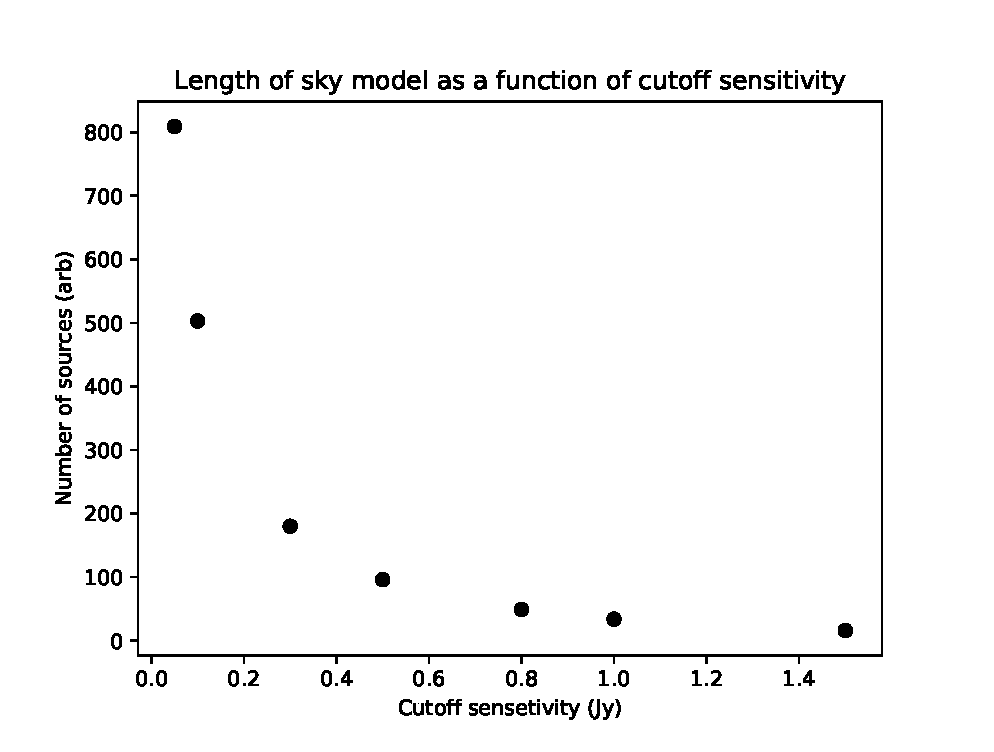
\includegraphics[width=0.8\linewidth]{ch6/figures/skymodel_size_vs_Jy.eps}
      \caption{The size of the sky model (measured in number of sources) increases exponentially as we decrease the flux cutoff of the model (i.e. increase the sensitivity).}
	\label{fig:ch6_skymodel_size}
\end{figure}


Finally, the number of CPU cores (henceforth just `CPUs') used by each step is a parameter that can be optimized for the entire pipeline. While increasing the number of CPUs can make some steps run faster, requesting jobs that reserve a large number of CPUs will take longer to launch on shared infrastructure. In order to understand the interplay between these effects, we study the queuing time and processing time as a function of the number of CPUs. For the parameter steps we choose to test 1, 2, 3, 4, 8 and 16 CPUs. 

\subsection{Infrastructure Performance}
%%%%%Staging files at different locations can be modelled using historical data, discuss the importance of knowing the time it takes to stage data and the prediction of future performance. 

In production, we run hundreds of LoTSS jobs on a cluster supporting several different use cases. The requested resources on this cluster are allocated by a job queue, in our case implemented by the glite workload management system \citep{glite-wms}. As queuing jobs can take a significant amount of time, we test the queuing time as a function of the number of requested CPUs. In order to do that, we create test jobs that log the launch time and submit them, requesting 1, 2, 3, 4, 8 and 16 CPUs. We run 10 to 15 tests for each parameter step to ensure that we capture system variability at different times of day during the week and the weekend. 

Besides queuing, time is also spent during downloading and unpacking data, as well as packing and uploading the results. Despite using no compression to pack the data, untarring and tarring large files still takes time depending on the system workload. We measure the time taken to transfer and unpack data of different sizes. The data sizes we chose were 0.5GB, 1GB, 2GB, 4GB, 8GB, 16GB, 32GB and 64GB. As our largest data sets are 64GB and our smallest results are $\sim$0.2GB, these values span a realistic range expected for LOFAR data processing. We test this by uploading mock data to the dCache storage pool at SURFsara and launching a small 1 CPU job on the cluster, which downloads and untars the data and logs the start time of each step. We present the results of this test in the next section. 


\subsubsection{Software Versions}\label{sec:ch6_software_versions}
For the current test, we use the LOFAR software stack, version 2.20.2 \citep{cookbook}. This software was compiled on a virtual machine and distributed using the CERN CVMFS virtually mounted file system \citep{cvmfs2008}. We use this software version and distribution method as it is the same software version and distribution used to process the data for the LOTSS Data Release 1. 

\subsection{Test Hardware}\label{sec:ch6_hardware}

We test the LOFAR software on a reserved node on the SURFsara \texttt{GINA} cluster. The node, f18-01 has 348 GB of RAM, 3TB of scratch space\footnote{More detailed specifications are at \href{http://docs.surfsaralabs.nl/projects/grid/en/latest/Pages/Service/system_specifications/gina_specs.html}{the \texttt{GINA} specification page linked here}}. The CPU is an Intel Xeon(R) Gold 6148 CPU with 40 cores clocked at 2.40GHz.  As this hardware node was reserved, there was no other scientific processing aside from our tests, meaning there was no resource contention aside for that inherent in the LOFAR software. In the results section, we compare these isolated runs with processing results over the past two years. 
